\newpage
\section{Grokking EA}
\visHeader

\vspace*{0.5cm}

\begin{quote} {\small Grok: ``\ldots to understand so thoroughly that the observer becomes a part of the observed.''\\
\hspace*{3.2cm} - Robert A. Heinlein, \emph{Stranger in a Strange land}}
\end{quote}

\vspace{0.5cm}

This section is a collection of a few of what we feel are the most important tips and tricks for working productively with EA. 
We truly believe that spending the time to learn and practice these is necessary for a pleasant modelling experience.

\vspace{0.5cm}

\section{Positioning elements}

Layout is always an important factor when using a visual language:
A well laid-out diagram is easiest to understand and, by centralizing important
elements or clustering related elements, you can actually impart additional information.

\begin{stepbystep}
\item To select a group of elements, either drag a selection box around the items or hold \texttt{Ctrl} and select each element
one-by-one.

\item In the top right corner of the last selected element, a small colon-styled symbol will appear (\Cref{ea:layout1}). Click on
this for a context list of different options you can simultaneously apply to all active elements. The same list appears on the toolbar above the
diagram. 

\item Experiment to find out what effect each option has. The last symbol in the list opens a further drop-down menu with standard layout
algorithms to organize your diagram automatically.

\item Right-clicking any of the selected elements opens a different menu with a further set of layout options and their descriptions
(\Cref{ea:layout2}). \texttt{Align Centers} or \texttt{Same Height and Width} can be especially useful.

\begin{figure}[htbp]
\begin{center} 
  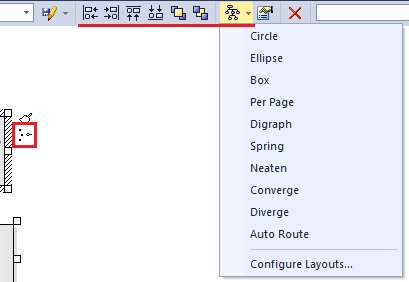
\includegraphics[width=0.65\textwidth]{../../org.moflon.doc.handbook.05_miscellaneous/1_grokkingEA/01_layOutElements/ea_layoutElementsCommonContext}
  \caption{Setting the layout of multiple elements}  
  \label{ea:layout1}
\end{center}
\end{figure}

\begin{figure}[htbp]
\begin{center}  
  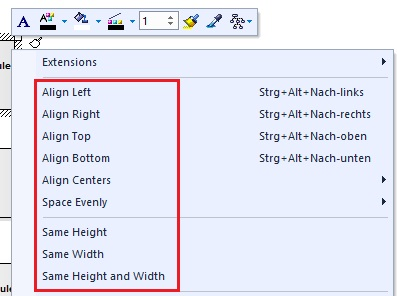
\includegraphics[width=0.7\textwidth]{../../org.moflon.doc.handbook.05_miscellaneous/1_grokkingEA/01_layOutElements/layoutElements2}
  \caption{Further layout options}  
  \label{ea:layout2} 
\end{center}
\end{figure}

\end{stepbystep}


\subsection{Bending lines to your will}

Almost as important as a good layout is getting lines to be just the way you want them to be. In EA you can add and remove bending points which can be used to
control the appearance of a line.

\begin{enumerate}
\item[$\blacktriangleright$]Hold down \texttt{Ctrl} and click on a line to create a bending point (Fig.~\ref{fig_bendLine01}). You can now pull and place the
bending point as you wish.
 
\begin{figure}[htbp]
\begin{center}
  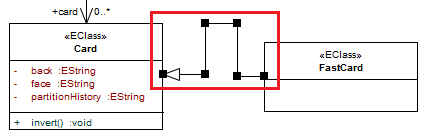
\includegraphics[width=0.8\textwidth]{bendLine1}
  \caption{How to bend lines}   
  \label{fig_bendLine01}
\end{center}
\end{figure}

\item[$\blacktriangleright$] You can create as many bending points as you wish, or \emph{remove} them also by holding down \texttt{Ctrl} and clicking on the
point to be deleted.
\end{enumerate}


\subsection{Deleting vs. removing elements from diagrams} 

A central feature that new users should understand as soon as possible is the way EA handles diagrams. \emph{A diagram is simply treated as a \emph{view} of the
complete model.} The complete model can always be browsed in its entirety via a tree view in the package browser. This space contains all elements that will be
exported. The driving reason behind this setup is that diagrams typically do not contain all elements and one usually uses multiple (possibly redundant)
diagrams to show the different parts of the model. Thinking in this frame is crucial and provides a pragmatic solution to the problem of having huge,
unmaintainable diagrams.

A tricky consequence one must get used to is that removing an element from a diagram does \emph{not} delete it from the model. We have added some support
with the validation in the eMoflon add-in control panel, which can prompt a warning when an element cannot be found in any diagram,\footnote{Review Part II,
Section 2.8 for an example} but there's currently no way to recover a deleted element.

A common mistake new users make is to remove an element by pressing \texttt{del}, and expecting the element to be deleted from the model. As you can probably
guess, this is not the case as evidenced in the package browser (Fig.~\ref{ea:partiallyDeleted}).

\vspace{0.5cm}

\begin{figure}[htbp]
\begin{center} 
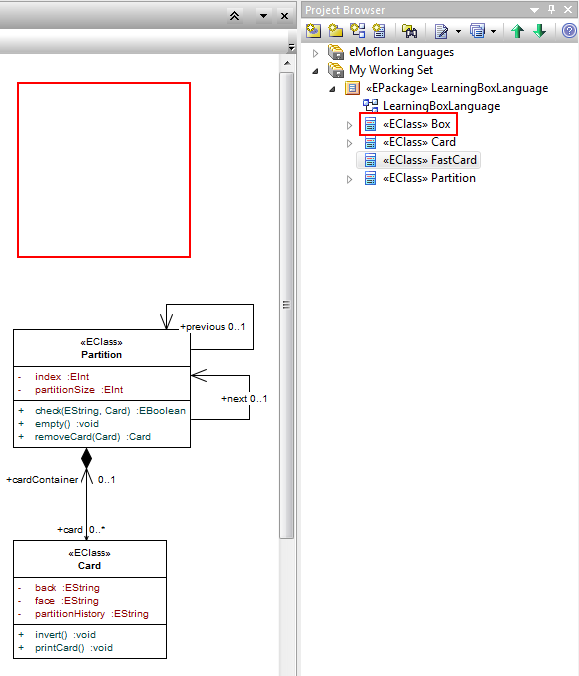
\includegraphics[width=0.6\textwidth]{ea_partiallyDeleted}
  \caption{Removing an element from a diagram via pressing \texttt{Del} does not delete it from the model and it is still present in the package browser}  
    \label{ea:partiallyDeleted}
\end{center}
\end{figure}  

\begin{itemize}
\item[$\blacktriangleright$] To fully delete an element from a model (not just a diagram), select it in the diagram and press \texttt{Ctrl + Del}. Confirm the
action in the warning dialogue (Fig.~\ref{ea:deleteWarning}), and the element should no longer be in the project browser.

\vspace{0.5cm}

\item[$\blacktriangleright$] Alternatively, elements can be deleted directly from project browser by right-clicking the item and navigating to the large
red `x' at the bottom of the context menu

\begin{figure}[htbp]
\begin{center}
  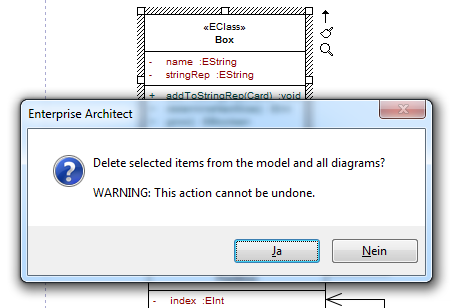
\includegraphics[width=0.7\textwidth]{ea_deleteWarning}
  \caption{Deleting an element from a diagram and the model}  
  \label{ea:deleteWarning}
\end{center}
\end{figure}  

\end{itemize}


\newpage
\subsection{Excluding certain projects from the export}

You may find it sometimes necessary to exclude certain projects from your diagram export (such as the \texttt{MocaTree} model used in Part V).
Some reasons for this could be (i) because the project is still a work in progress and simply not ready to be exported, (ii) because the
complete project is present in the Eclipse workspace but has not been modelled completely in EA, and you wish to do this gradually on-demand, (iii) because the
project is not meant to be present in your Eclipse workspace as generated code and is instead provided via a plugin (this is usually the case for standard
metamodels like Ecore, UML etc.), or (iv) because the project is rather large and stable and you do not want to wait for EA to process a known, unchanging
model. Whatever the reason, you can prevent unnecessary exports by setting a certain \emph{tagged value} of the project.

\begin{enumerate}

\item[$\blacktriangleright$] Open your project in EA, and navigate to ``View/Tagged Values'' from the menu bar (Fig.~\ref{ea:view/Taggedvalues}).

\begin{figure}[htbp]
\begin{center}  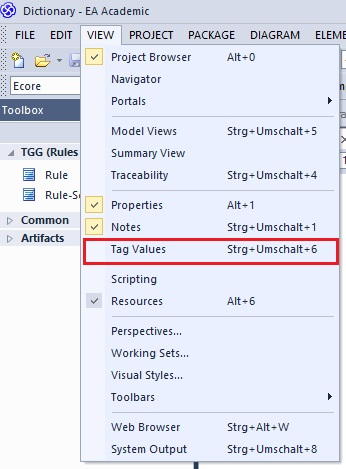
\includegraphics[width=0.5\textwidth]{ea_viewTaggedValues}
  \caption{Opening the tagged values view}  
  \label{ea:view/Taggedvalues}
\end{center}
\end{figure} 

\item[$\blacktriangleright$] The tagged value, \emph{Moflon::Export}, should already be present and be set to a default \texttt{true} value
(Fig.~\ref{ea:moflonExportTG}). If you want the project to be ignored by the eMoflon's validation and/or export functions, change the value to
\texttt{false} (and conversely back to \texttt{true} to export it again).

\begin{figure}[htbp]
\begin{center}
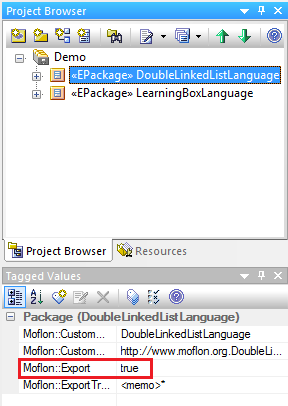
\includegraphics[width=0.5\textwidth]{ea_moflonExportTG}
  \caption{The \texttt{Moflon::Export} setting determines ignored projects}  
  \label{ea:moflonExportTG}
\end{center}
\end{figure}

\end{enumerate}


\subsection{Getting verbose!}

Although we use colours in SDMs to indicate when an element is to be matched (black), created (green), or destroyed (red), it sometimes makes sense to
indicate these binding operators via explicit stereotypes (i.e., for black-and-white printouts of a model).

\begin{enumerate}
  
\item[$\blacktriangleright$] Open the relevant diagram in the EA editor window and, depending on what type it is, press the \texttt{Verbose} button in
either the \texttt{eMoflon SDM Functions} or \texttt{eMoflon TGG Functions} panel (Fig.~\ref{ea:changeVStatus}).

\vspace{0.5cm}

\begin{figure}[htbp]
\begin{center}
  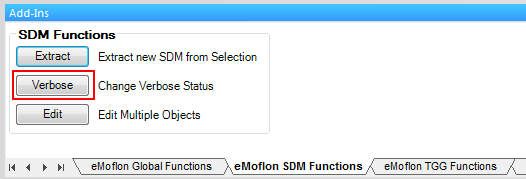
\includegraphics[width=0.8\textwidth]{ea_changeVerboseStatus}
  \caption{Add extra markup to colored links and objects in the current diagram}  
  \label{ea:changeVStatus}
\end{center}
\end{figure}

\item[$\blacktriangleright$] This will add small \texttt{++} or \texttt{-~-} symbols next to deleted and created elements in the current diagram
(Fig.~\ref{ea:verboseSymbols}). Press the button again to deactivate these indicators.

\begin{figure}[htbp]
\begin{center}
  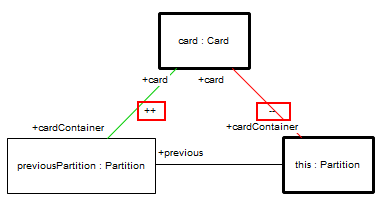
\includegraphics[width=0.7\textwidth]{ea_verboseSymbols}
  \caption{Diagram in verbose mode}  
  \label{ea:verboseSymbols}
\end{center}
\end{figure}

\end{enumerate}


\newpage

\subsection{Duplicating elements via drag-and-drop}

Sometimes you'll have an element (or many) that are nearly identical, and life would be \emph{so} much easier if you could copy and paste an existing one
already. Suppose you want a copy of a \emph{this} element, so you press \texttt{ctrl + C}, followed by \texttt{ctrl + v}. An error dialogue preventing the
action will immediately raise, stating that the ``\ldots diagram already contains an instance of the element you are trying to paste.'' EA can only support
unique objects, so you'll need to use the following process.

\begin{itemize}

\item[$\blacktriangleright$] In either a diagram or in the project browser, hold \texttt{ctrl}, then drag the element you wish to duplicate. A
confirmation-style dialogue will appear (Fig.~\ref{ea:dupWindow}), and a properties window will follow. You must assign a unique name to the new element, or
else you'll receive an error when you try to export the project later.

\begin{figure}[htbp]
\begin{center}
  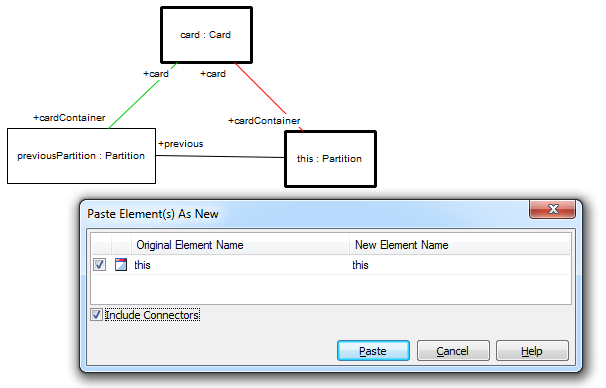
\includegraphics[width=0.95\textwidth]{ea_duplicatingElements}
  \caption{Copying new elements}  
  \label{ea:dupWindow}
\end{center}
\end{figure}

\end{itemize}


\newpage

\hypertarget{subsec:seekAndFind}{}

\subsection{Seek, and ye shall find \ldots}

EA has a model search function that can be quite handy for large models with thousands of elements and a brain that just can't remember where something is. 

\begin{enumerate}

\item[$\blacktriangleright$]Select ``Model Search Window'' and enter the name of an element you wish to find (Fig.~\ref{fig_search01}).\footnote{You can also
access this window by pressing \texttt{ctrl+alt+A}} 

\begin{figure}[htbp]
\begin{center}
  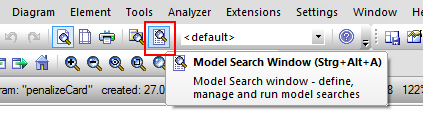
\includegraphics[width=0.63\textwidth]{search1}
  \caption{Model Search Window}  
  \label{fig_search01}
\end{center}
\end{figure}

\item[$\blacktriangleright$] All elements that meet the search criteria are listed and you can right-click on each of the items and select one of the options
above to locate the element.

\item[$\blacktriangleright$] In a similar way, you can locate the corresponding class of an object by right clicking and selecting ``Find/Locate Classifier in
Project Browser.''

\end{enumerate}


\subsection{Advanced search}
\label{sect:appendix_adv_search}

EA offers an even more advanced search capability using SQL\footnote{For some detailed insights to the general database schema used by EA cf. \\
\url{http://www.sparxsystems.com.au/downloads/corp/scripts/SQLServer_EASchema.sql}}.
To make use of this option, go to the model search dialog (\mbox{Ctrl+Alt+A}). Click on the ``Builder'' button and switch to the SQL-tab. Here you can 
formulate any query on the underlying database. The SQL-editor helps you with syntax-highlighting and auto-completion. Here are some basic examples:

\begin{enumerate}
\item[$\blacktriangleright$]
To find all eClasses
\begin{lstlisting}[frame=single,framerule=0pt]
SELECT * FROM t_object
WHERE Object_Type='Class' AND Stereotype='eclass';
\end{lstlisting}

\item[$\blacktriangleright$]
To find all associations
\begin{lstlisting}[frame=single,framerule=0pt]
SELECT * FROM t_connector
WHERE Connector_Type='Association';
\end{lstlisting}

\item[$\blacktriangleright$]
To find all inheritance relations
\begin{lstlisting}[frame=single,framerule=0pt]
SELECT * FROM t_connector
WHERE Connector_Type='Generalization';
\end{lstlisting}

\item[$\blacktriangleright$]
To find all connectors attaching a note to an element
\begin{lstlisting}[frame=single,framerule=0pt]
SELECT * FROM t_connector
WHERE Connector_Type='NoteLink';
\end{lstlisting}

\item[$\blacktriangleright$]
To find all control flow edges (used in SDMs)
\begin{lstlisting}[frame=single,framerule=0pt]
SELECT * FROM t_connector
WHERE Connector_Type='ControlFlow';
\end{lstlisting}

\item[$\blacktriangleright$]
To find all associations connected to a class named ``EClass''
\begin{lstlisting}[frame=single,framerule=0pt]
SELECT t_object.Name, t_connector.* FROM t_connector,t_object
WHERE t_connector.Connector_Type='Association'
  AND (t_connector.Start_Object_ID=t_object.Object_ID
    OR t_connector.End_Object_ID=t_object.Object_ID)
  AND t_object.Name='EClass';
\end{lstlisting}

\item[$\blacktriangleright$]
To determine all subtypes of ``EClassifier''
\begin{lstlisting}[frame=single,framerule=0pt]
SELECT a.Name FROM t_connector,t_object a,t_object b
WHERE t_connector.Connector_Type='Generalization'
  AND t_connector.Start_Object_ID=a.Object_ID
  AND t_connector.End_Object_ID=b.Object_ID
  AND b.Name = 'EClassifier';
\end{lstlisting}

\item[$\blacktriangleright$]
To determine all supertypes of ``EClassifier'' (cf. above)
\begin{lstlisting}[frame=single,framerule=0pt]
...
  AND t_connector.Start_Object_ID=b.Object_ID
  AND t_connector.End_Object_ID=a.Object_ID
...
\end{lstlisting}
\end{enumerate}

To run the search, either hit the run button in the upper left corner of the editor (it shows a triangular shaped ``play'' pictogram) or punch \texttt{F5} on
your keyboard.

\clearpage
